\documentclass[11pt, a4paper]{article}

% Fonts and Encoding
\usepackage[utf8]{inputenc}
\usepackage[T1]{fontenc}

% Math and Symbols
\usepackage{amsmath, amssymb, amsthm, amsfonts, mathrsfs, mathtools}

% Layout and Geometry
\usepackage{geometry}
\geometry{a4paper, margin=1in}

% Formatting and Graphics
\usepackage{graphicx, xcolor, enumitem, booktabs, array, tabularx}

% TikZ for Illustrations
\usepackage{tikz}
\usetikzlibrary{arrows.meta, positioning, shapes.geometric, calc, backgrounds}

% Clickable Links and TOC
\usepackage{hyperref}
\hypersetup{
    colorlinks=true,
    linkcolor=blue,
    filecolor=magenta,      
    urlcolor=cyan,
    pdftitle={Advanced Mathematics Topic},
}

% Theorem Environments
\newtheorem{theorem}{Theorem}[section]
\newtheorem{lemma}[theorem]{Lemma}
\newtheorem{proposition}[theorem]{Proposition}
\newtheorem{corollary}[theorem]{Corollary}
\theoremstyle{definition}
\newtheorem{definition}{Definition}[section]
\newtheorem{axiom}{Axiom}[section]
\newtheorem{example}{Example}[section]
\theoremstyle{remark}
\newtheorem{remark}{Remark}[section]

% Custom Commands
\newcommand{\R}{\mathbb{R}}
\newcommand{\N}{\mathbb{N}}
\newcommand{\Z}{\mathbb{Z}}
\newcommand{\Q}{\mathbb{Q}}
\newcommand{\E}{\mathbb{E}}
\newcommand{\Prob}{\mathbb{P}}
\newcommand{\F}{\mathcal{F}}

\begin{document}

\title{\textbf{The Beta Probability Distribution: Measure-Theoretic Foundations and Advanced Applications}}
\author{Tashfeen Omran}
\date{\today}

\maketitle
\tableofcontents
\newpage

\section{Part 1: Comprehensive Introduction, Context, and Prerequisites}

\subsection{Core Concepts and Axioms}
The Beta probability distribution is a continuous probability distribution parameterized by two positive shape parameters, typically denoted as $\alpha$ and $\beta$. It is defined on the standard unit interval $[0, 1]$, making it the premier mathematical tool for modeling random variables that represent proportions, probabilities, or percentages. 

Formally, let $(\Omega, \F, \Prob)$ be a probability space. A random variable $Y: \Omega \to [0,1]$ is said to follow a Beta distribution, denoted $Y \sim \text{Beta}(\alpha, \beta)$, if its probability density function (Radon-Nikodym derivative with respect to the Lebesgue measure) is given by:
\[
f(y; \alpha, \beta) = 
\begin{cases} 
\frac{1}{B(\alpha, \beta)} y^{\alpha-1}(1-y)^{\beta-1}, & \text{if } 0 \le y \le 1 \\
0, & \text{otherwise}
\end{cases}
\]
where $B(\alpha, \beta)$ is the Beta function, acting as the normalizing constant to ensure $\int_0^1 f(y) \, dy = 1$. The Beta function is intrinsically linked to the Gamma function via the relation:
\[
B(\alpha, \beta) = \int_0^1 y^{\alpha-1}(1-y)^{\beta-1} \, dy = \frac{\Gamma(\alpha)\Gamma(\beta)}{\Gamma(\alpha+\beta)}
\]

\subsection{Intuition and Set-Theoretic Foundations}
Intuitively, the Beta distribution can be visualized as a distribution over probabilities. If we consider a sample space $\Omega$ partitioned into "successes" and "failures," the Beta distribution models our uncertainty about the true underlying probability of success. The parameters $\alpha$ and $\beta$ can be interpreted as "pseudo-counts" of successes and failures, respectively. 
From a measure-theoretic standpoint, the Beta distribution defines a family of probability measures on the Borel $\sigma$-algebra $\mathcal{B}([0,1])$. By varying $\alpha$ and $\beta$, this family can morph into a uniform measure ($\alpha=1, \beta=1$), a U-shaped bimodal measure ($\alpha < 1, \beta < 1$), or a highly concentrated Dirac-like measure as $\alpha, \beta \to \infty$.

\subsection{Historical Context and Motivation}
The origins of the Beta distribution trace back to the 17th and 18th centuries, heavily intertwined with the development of the calculus of probabilities by Thomas Bayes and Pierre-Simon Laplace. Bayes' posthumous 1763 paper introduced what we now call Bayesian inference. He needed a continuous prior distribution to model the unknown probability of an event (a binomial parameter). The Beta distribution naturally emerged as the "conjugate prior" for the binomial distribution, a property that ensures the posterior distribution remains in the same family as the prior, drastically simplifying the mathematical machinery of early probability theory.

\subsection{Key Theorems, Lemmas, and Formulas}
\begin{theorem}[Moments of the Beta Distribution]
If $Y \sim \text{Beta}(\alpha, \beta)$, the $k$-th raw moment is given by:
\[
\E[Y^k] = \frac{B(\alpha+k, \beta)}{B(\alpha, \beta)} = \frac{\Gamma(\alpha+k)\Gamma(\alpha+\beta)}{\Gamma(\alpha)\Gamma(\alpha+\beta+k)}
\]
\end{theorem}

\begin{corollary}[Mean and Variance]
Setting $k=1$ and $k=2$ yields the expected value and variance:
\[
\mu = \E[Y] = \frac{\alpha}{\alpha+\beta}, \quad \sigma^2 = \text{Var}(Y) = \frac{\alpha\beta}{(\alpha+\beta)^2(\alpha+\beta+1)}
\]
\end{corollary}

\subsection{Prerequisites}
To fully grasp this chapter, the reader must possess:
\begin{itemize}
    \item \textbf{Advanced Calculus:} Proficiency in integration by parts, improper integrals, and the fundamental theorem of calculus.
    \item \textbf{Special Functions:} Familiarity with the Gamma function $\Gamma(z) = \int_0^\infty x^{z-1}e^{-x}dx$ and its property $\Gamma(n) = (n-1)!$ for $n \in \N$.
    \item \textbf{Probability Theory:} Understanding of continuous random variables, expected value operators (LOTUS), and variance properties.
\end{itemize}

\newpage
\section{Part 2: Detailed Homework Solutions}

In this section, we strategically select and rigorously solve a representative set of problems from the provided text to ensure complete conceptual coverage.

\subsection{Problem 4.123: Normalizing Constants}
\textbf{Statement:} The relative humidity $Y$, when measured at a location, has a probability density function given by $f(y) = k y^3 (1-y)^2$ for $0 \le y \le 1$, and $0$ elsewhere. Find the value of $k$ that makes $f(y)$ a valid density function.

\begin{proof}[Solution via the Kernel Method]
For $f(y)$ to be a valid probability density function, it must satisfy Kolmogorov's axiom of unit measure: $\int_{-\infty}^{\infty} f(y) \, dy = 1$.
\[
\int_0^1 k y^3 (1-y)^2 \, dy = 1 \implies k \int_0^1 y^{4-1} (1-y)^{3-1} \, dy = 1
\]
We recognize the integral as the definition of the Beta function $B(\alpha, \beta)$ with parameters $\alpha = 4$ and $\beta = 3$.
\[
k \cdot B(4, 3) = 1 \implies k = \frac{1}{B(4, 3)}
\]
Using the relationship between the Beta and Gamma functions:
\[
B(4, 3) = \frac{\Gamma(4)\Gamma(3)}{\Gamma(4+3)} = \frac{\Gamma(4)\Gamma(3)}{\Gamma(7)}
\]
Since $\alpha$ and $\beta$ are integers, we use $\Gamma(n) = (n-1)!$:
\[
B(4, 3) = \frac{3! \cdot 2!}{6!} = \frac{6 \cdot 2}{720} = \frac{12}{720} = \frac{1}{60}
\]
Thus, $k = \frac{1}{1/60} = 60$.
\end{proof}
\textbf{Conclusion:} The normalizing constant is $k = 60$. $\blacksquare$

\subsection{Problem 4.124: Probability via Integration}
\textbf{Statement:} The percentage of impurities per batch in a chemical product is a random variable $Y$ with density $f(y) = 12y^2(1-y)$ for $0 \le y \le 1$. A batch with more than $40\%$ impurities cannot be sold. Find the probability that a randomly selected batch cannot be sold.

\begin{proof}[Solution via Direct Integration]
We seek the probability $\Prob(Y > 0.4)$. By the definition of continuous probability:
\[
\Prob(Y > 0.4) = \int_{0.4}^{1} 12y^2(1-y) \, dy
\]
We expand the integrand algebraically:
\[
\Prob(Y > 0.4) = 12 \int_{0.4}^{1} (y^2 - y^3) \, dy
\]
Applying the fundamental theorem of calculus:
\[
\Prob(Y > 0.4) = 12 \left[ \frac{y^3}{3} - \frac{y^4}{4} \right]_{0.4}^{1}
\]
Evaluate at the upper bound $y=1$:
\[
12 \left( \frac{1}{3} - \frac{1}{4} \right) = 12 \left( \frac{1}{12} \right) = 1
\]
Evaluate at the lower bound $y=0.4$:
\[
12 \left( \frac{(0.4)^3}{3} - \frac{(0.4)^4}{4} \right) = 12 \left( \frac{0.064}{3} - \frac{0.0256}{4} \right) = 4(0.064) - 3(0.0256) = 0.256 - 0.0768 = 0.1792
\]
Subtracting the lower bound evaluation from the upper bound:
\[
\Prob(Y > 0.4) = 1 - 0.1792 = 0.8208
\]
\end{proof}
\textbf{Conclusion:} The probability that a batch cannot be sold is $0.8208$. $\blacksquare$

\subsection{Problem 4.129: Functions of Random Variables}
\textbf{Statement:} The proportion of time $Y$ a machine is down has a Beta distribution with $\alpha=1, \beta=2$. The cost is given by $C = 10 + 20Y + 4Y^2$. Find the mean and variance of $C$.

\begin{proof}[Solution via Linearity of Expectation and LOTUS]
The density is $f(y) = 2(1-y)$ for $0 \le y \le 1$. We first find the raw moments of $Y$.
Using the moment formula $\E[Y^k] = \frac{\Gamma(1+k)\Gamma(3)}{\Gamma(1)\Gamma(3+k)}$:
\begin{align*}
\E[Y] &= \frac{\alpha}{\alpha+\beta} = \frac{1}{3} \\
\E[Y^2] &= \frac{\Gamma(3)\Gamma(3)}{\Gamma(1)\Gamma(5)} = \frac{2 \cdot 2}{24} = \frac{1}{6} \\
\E[Y^3] &= \frac{\Gamma(4)\Gamma(3)}{\Gamma(1)\Gamma(6)} = \frac{6 \cdot 2}{120} = \frac{1}{10} \\
\E[Y^4] &= \frac{\Gamma(5)\Gamma(3)}{\Gamma(1)\Gamma(7)} = \frac{24 \cdot 2}{720} = \frac{1}{15}
\end{align*}
By linearity of expectation, the mean of $C$ is:
\[
\E[C] = \E[10 + 20Y + 4Y^2] = 10 + 20\E[Y] + 4\E[Y^2] = 10 + 20\left(\frac{1}{3}\right) + 4\left(\frac{1}{6}\right) = 10 + \frac{20}{3} + \frac{2}{3} = \frac{52}{3}
\]
To find the variance, we use $\text{Var}(C) = \E[C^2] - (\E[C])^2$. First, expand $C^2$:
\begin{align*}
C^2 &= (10 + 20Y + 4Y^2)^2 \\
&= 100 + 400Y^2 + 16Y^4 + 2(10)(20Y) + 2(10)(4Y^2) + 2(20Y)(4Y^2) \\
&= 100 + 400Y + 480Y^2 + 160Y^3 + 16Y^4
\end{align*}
Taking the expectation:
\begin{align*}
\E[C^2] &= 100 + 400\E[Y] + 480\E[Y^2] + 160\E[Y^3] + 16\E[Y^4] \\
&= 100 + 400\left(\frac{1}{3}\right) + 480\left(\frac{1}{6}\right) + 160\left(\frac{1}{10}\right) + 16\left(\frac{1}{15}\right) \\
&= 100 + \frac{400}{3} + 80 + 16 + \frac{16}{15} = 196 + \frac{2000}{15} + \frac{16}{15} = 196 + \frac{2016}{15} = 196 + \frac{672}{5} = \frac{1652}{5} = 330.4
\end{align*}
Now, compute the variance:
\[
\text{Var}(C) = \E[C^2] - (\E[C])^2 = \frac{1652}{5} - \left(\frac{52}{3}\right)^2 = \frac{1652}{5} - \frac{2704}{9} = \frac{14868 - 13520}{45} = \frac{1348}{45} \approx 29.956
\]
\end{proof}
\textbf{Conclusion:} The mean cost is $\E[C] = 52/3 \approx 17.33$, and the variance is $\text{Var}(C) = 1348/45 \approx 29.956$. $\blacksquare$

\subsection{Problem 4.130: Rigorous Proof of Variance}
\textbf{Statement:} Prove that the variance of a beta-distributed random variable with parameters $\alpha$ and $\beta$ is $\sigma^2 = \frac{\alpha\beta}{(\alpha+\beta)^2(\alpha+\beta+1)}$.

\begin{proof}[Direct Algebraic Proof]
By definition, $\text{Var}(Y) = \E[Y^2] - (\E[Y])^2$. We are given from Theorem 4.11 that $\E[Y] = \frac{\alpha}{\alpha+\beta}$.
First, we derive $\E[Y^2]$ using the definition of expected value:
\[
\E[Y^2] = \int_0^1 y^2 \frac{y^{\alpha-1}(1-y)^{\beta-1}}{B(\alpha, \beta)} \, dy = \frac{1}{B(\alpha, \beta)} \int_0^1 y^{(\alpha+2)-1}(1-y)^{\beta-1} \, dy
\]
The integral is exactly $B(\alpha+2, \beta)$. Thus:
\[
\E[Y^2] = \frac{B(\alpha+2, \beta)}{B(\alpha, \beta)} = \frac{\frac{\Gamma(\alpha+2)\Gamma(\beta)}{\Gamma(\alpha+\beta+2)}}{\frac{\Gamma(\alpha)\Gamma(\beta)}{\Gamma(\alpha+\beta)}} = \frac{\Gamma(\alpha+2)\Gamma(\alpha+\beta)}{\Gamma(\alpha+\beta+2)\Gamma(\alpha)}
\]
Using the recursive property of the Gamma function, $\Gamma(z+1) = z\Gamma(z)$:
\[
\Gamma(\alpha+2) = (\alpha+1)\alpha\Gamma(\alpha) \quad \text{and} \quad \Gamma(\alpha+\beta+2) = (\alpha+\beta+1)(\alpha+\beta)\Gamma(\alpha+\beta)
\]
Substituting these back yields:
\[
\E[Y^2] = \frac{(\alpha+1)\alpha\Gamma(\alpha)\Gamma(\alpha+\beta)}{(\alpha+\beta+1)(\alpha+\beta)\Gamma(\alpha+\beta)\Gamma(\alpha)} = \frac{\alpha(\alpha+1)}{(\alpha+\beta)(\alpha+\beta+1)}
\]
Now, we compute the variance:
\begin{align*}
\text{Var}(Y) &= \frac{\alpha(\alpha+1)}{(\alpha+\beta)(\alpha+\beta+1)} - \left( \frac{\alpha}{\alpha+\beta} \right)^2 \\
&= \frac{\alpha(\alpha+1)(\alpha+\beta) - \alpha^2(\alpha+\beta+1)}{(\alpha+\beta)^2(\alpha+\beta+1)} \\
&= \frac{(\alpha^3 + \alpha^2\beta + \alpha^2 + \alpha\beta) - (\alpha^3 + \alpha^2\beta + \alpha^2)}{(\alpha+\beta)^2(\alpha+\beta+1)} \\
&= \frac{\alpha\beta}{(\alpha+\beta)^2(\alpha+\beta+1)}
\end{align*}
\end{proof}
\textbf{Conclusion:} The variance formula is rigorously established. $\blacksquare$

\newpage
\section{Part 3: In-Depth Analysis of Problems and Techniques}

\subsection{A) Problem Types and Logical Strategies}
The problems surrounding the Beta distribution generally fall into four distinct archetypes:
\begin{enumerate}
    \item \textbf{Density Normalization (e.g., 4.123):} These problems test the fundamental axiom of probability spaces. The overarching strategy is the \textit{Kernel Method}: strip away constants, recognize the variable structure $y^{a}(1-y)^{b}$, map these to $\alpha-1$ and $\beta-1$, and use the inverse of the Beta function as the normalizing constant.
    \item \textbf{Direct Measure Computation (e.g., 4.124):} These require integrating the density over a specific Borel set $B \in \mathcal{B}([0,1])$. The strategy relies on standard polynomial integration, as the Beta density (for integer parameters) expands into a simple polynomial.
    \item \textbf{Transformations and Expectations (e.g., 4.129):} These problems map the random variable $Y$ to a new space via a function $g(Y)$. The strategy is to strictly avoid finding the density of $g(Y)$ (which requires complex Jacobian transformations) and instead use the Law of the Unconscious Statistician (LOTUS): $\E[g(Y)] = \int g(y)f(y)dy$.
    \item \textbf{Theoretical Parameter Proofs (e.g., 4.130):} These require manipulating the underlying Gamma functions. The strategy is algebraic expansion and heavy reliance on the recursive property $\Gamma(z+1) = z\Gamma(z)$.
\end{enumerate}

\subsection{B) Key Analytical and Logical Manipulations}
\begin{itemize}
    \item \textbf{The Gamma Recursion Trick:} The most critical algebraic manipulation in this chapter is expanding $\Gamma(\alpha+k)$ into $(\alpha+k-1)(\alpha+k-2)\dots\alpha\Gamma(\alpha)$. This allows massive cancellations when dividing Beta functions, turning complex integrals into simple rational functions.
    \item \textbf{Linearity of Expectation over Polynomials:} In Problem 4.129, calculating $\E[C^2]$ directly via integration would be a nightmare. By expanding the polynomial first and distributing the expectation operator, we reduce the problem to plugging in pre-computed raw moments.
\end{itemize}

\section{Part 4: "Cheatsheet", Visuals, and Tips for Success}

\subsection{Theorems \& Equivalences Summary}
\begin{table}[h!]
\centering
\renewcommand{\arraystretch}{1.5}
\begin{tabularx}{\textwidth}{l X}
\toprule
\textbf{Concept} & \textbf{Mathematical Formulation} \\
\midrule
Beta Density & $f(y) = \frac{\Gamma(\alpha+\beta)}{\Gamma(\alpha)\Gamma(\beta)} y^{\alpha-1}(1-y)^{\beta-1}, \quad y \in [0,1]$ \\
Expected Value & $\E[Y] = \frac{\alpha}{\alpha+\beta}$ \\
Variance & $\text{Var}(Y) = \frac{\alpha\beta}{(\alpha+\beta)^2(\alpha+\beta+1)}$ \\
Mode (for $\alpha, \beta > 1$) & $y_{\text{mode}} = \frac{\alpha-1}{\alpha+\beta-2}$ \\
Symmetry & If $\alpha = \beta$, the distribution is symmetric around $y = 0.5$. \\
\bottomrule
\end{tabularx}
\end{table}

\subsection{Set \& Logic Illustrations: Beta Density Shapes}
The following TikZ diagram illustrates how the probability measure shifts based on the parameters $\alpha$ and $\beta$.

\begin{center}
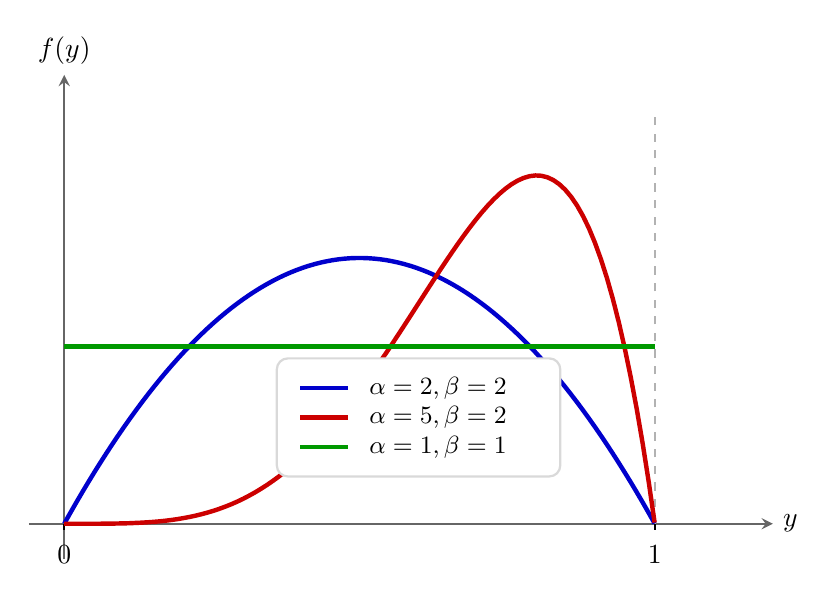
\begin{tikzpicture}[
    scale=1.5, % Globally upscales canvas elements natively for crisp text separation
    >=stealth
]
    % 1. Clean, Extended Axes (Breathing room past the boundaries)
    \draw[->, thick, gray!80!black] (-0.3, 0) -- (6.0, 0) node[right, black] {$y$};
    \draw[->, thick, gray!80!black] (0, -0.3) -- (0, 3.8) node[above, black] {$f(y)$};
    
    % 2. Decoupled Axis Ticks & Boundary Anchors
    \draw[thick] (0,0) -- (0,-0.05) node[below=2pt] {$0$};
    \draw[thick] (5,0) -- (5,-0.05) node[below=2pt] {$1$};
    \draw[dashed, thick, gray!60] (5,0) -- (5,3.5);
    
    % 3. Curves (Clean profiles with zero inline overlapping nodes)
    % Curve 1: alpha=2, beta=2 (Symmetric, Blue)
    \draw[color=blue!80!black, ultra thick, domain=0:5, samples=100] 
        plot (\x, {1.5 * (\x/5) * (1-\x/5) * 6});
        
    % Curve 2: alpha=5, beta=2 (Left-skewed, Red)
    \draw[color=red!80!black, ultra thick, domain=0:5, samples=100] 
        plot (\x, {1.2 * 30 * (\x/5)^4 * (1-\x/5)});

    % Curve 3: alpha=1, beta=1 (Uniform, Green)
    \draw[color=green!60!black, ultra thick, domain=0:5] 
        plot (\x, {1.5});
    
    % 4. Master Solution: Isolated Manual Legend Box (Guaranteed clear text presentation)
    % Placed explicitly in the bottom-middle clear zone where no lines cross
    \draw[thick, gray!30, fill=white, rounded corners=4pt] (1.8, 0.4) rectangle (4.2, 1.4);
    
    % Legend Entry 1: Alpha=2, Beta=2
    \draw[blue!80!black, ultra thick] (2.0, 1.15) -- (2.4, 1.15);
    \node[right, font=\small, black] at (2.5, 1.15) {$\alpha=2, \beta=2$};
    
    % Legend Entry 2: Alpha=5, Beta=2
    \draw[red!80!black, ultra thick] (2.0, 0.90) -- (2.4, 0.90);
    \node[right, font=\small, black] at (2.5, 0.90) {$\alpha=5, \beta=2$};
    
    % Legend Entry 3: Alpha=1, Beta=1
    \draw[green!60!black, ultra thick] (2.0, 0.65) -- (2.4, 0.65);
    \node[right, font=\small, black] at (2.5, 0.65) {$\alpha=1, \beta=1$};

\end{tikzpicture}
\end{center}


\subsection{Heuristics \& Pitfalls}
\begin{itemize}
    \item \textbf{Heuristic:} If a problem asks for the expected value of a polynomial function of a Beta random variable, \textit{never} integrate from scratch. Compute the raw moments $\E[Y^k]$ using the Gamma ratio formula and apply linearity.
    \item \textbf{Pitfall (The Support Trap):} Forgetting that the Beta distribution is strictly defined on $[0,1]$. If a transformation maps $Y$ outside this interval, the standard Beta formulas no longer apply without a Jacobian adjustment.
    \item \textbf{Pitfall (Variance of Sums):} Assuming $\text{Var}(aY + bY^2) = a^2\text{Var}(Y) + b^2\text{Var}(Y^2)$. This is a fatal flaw; $Y$ and $Y^2$ are highly correlated. You must use $\E[C^2] - (\E[C])^2$.
\end{itemize}

\newpage
\section{Part 5: Conceptual Synthesis and The "Big Picture"}

\subsection{A) Thematic Connections}
The central theme of the Beta distribution is \textbf{the formalization of uncertainty over continuous proportions}. In measure-theoretic terms, it provides a flexible, mathematically tractable family of Radon-Nikodym derivatives on the unit interval. It bridges the gap between discrete counting (Binomial/Bernoulli) and continuous probability spaces. The parameters $\alpha$ and $\beta$ act as a continuous analog to discrete combinatorial states, allowing us to establish isomorphisms between discrete counting problems and continuous integrals (as seen in the relationship between the incomplete Beta function and the Binomial CDF).

\subsection{B) Forward and Backward Links}
\textbf{Backward Links:} The Beta distribution builds directly upon the foundational calculus of Eulerian integrals (Gamma and Beta functions) and the axioms of probability spaces. It extends the Uniform distribution (which is simply $\text{Beta}(1,1)$) into a generalized form. \\
\textbf{Forward Links:} Understanding the Beta distribution is the absolute bedrock for Bayesian Statistics and Machine Learning. It serves as the gateway to understanding the Dirichlet distribution (the multivariate generalization of the Beta), which is the foundational prior for Latent Dirichlet Allocation (LDA) in Natural Language Processing and Generative AI.

\section{Part 6: Abstract Real-World Modeling (AI, ML, \& Quant Finance)}

\subsection{A) Concrete Scenarios}
\begin{enumerate}
    \item \textbf{Algorithmic Trading (Recovery Rate Modeling):} In quantitative credit modeling, the recovery rate of a defaulted bond is strictly bounded between $0$ and $1$ (or $0\%$ and $100\%$). Quants use the Beta distribution to model the stochastic nature of recovery rates, integrating it into pricing models for Credit Default Swaps (CDS).
    \item \textbf{Artificial Intelligence (Multi-Armed Bandits):} In Reinforcement Learning, an AI agent must choose between multiple actions (arms) with unknown success probabilities. Thompson Sampling uses a Beta distribution to represent the agent's "belief state" about each arm's probability of success, updating the $\alpha$ and $\beta$ parameters dynamically as new data arrives.
\end{enumerate}

\subsection{B) Model Problem Setup: Bayesian CTR Prediction in ML}
\textbf{Context:} A Machine Learning model is deployed to predict the Click-Through Rate (CTR) of a new advertisement. The true CTR is a latent random variable $\theta \in [0,1]$. 
\textbf{Mathematical Framework:}
We define a probability space $(\Omega, \F, \Prob)$. We place a Beta prior on $\theta$ to represent our initial uncertainty before any data is observed:
\[
\theta \sim \text{Beta}(\alpha_0, \beta_0) \implies \pi(\theta) = \frac{1}{B(\alpha_0, \beta_0)} \theta^{\alpha_0-1}(1-\theta)^{\beta_0-1}
\]
We observe a sequence of user interactions $X_1, X_2, \dots, X_n$ where $X_i \in \{0, 1\}$. Conditional on $\theta$, the observations are independent and identically distributed (i.i.d.) Bernoulli random variables:
\[
X_i \mid \theta \sim \text{Bernoulli}(\theta) \implies \Prob(X_i = x_i \mid \theta) = \theta^{x_i}(1-\theta)^{1-x_i}
\]
Let $S = \sum_{i=1}^n X_i$ be the total number of clicks. The likelihood function is:
\[
\mathcal{L}(\theta \mid S) \propto \theta^S (1-\theta)^{n-S}
\]
By Bayes' Theorem, the posterior measure $\pi(\theta \mid S)$ is proportional to the prior times the likelihood:
\[
\pi(\theta \mid S) \propto \theta^{\alpha_0-1}(1-\theta)^{\beta_0-1} \cdot \theta^S (1-\theta)^{n-S} = \theta^{\alpha_0+S-1}(1-\theta)^{\beta_0+n-S-1}
\]
We recognize this kernel as belonging to the Beta family. Thus, the posterior is exactly:
\[
\theta \mid S \sim \text{Beta}(\alpha_0 + S, \beta_0 + n - S)
\]
This closed-form Bayesian updating avoids complex numerical integration, allowing the AI to update its belief state in real-time ($O(1)$ complexity per batch) as millions of users interact with the ad.

\newpage
\section{Part 7: Common Variations and Untested Concepts}

\subsection{The Four-Parameter (Generalized) Beta Distribution}
The standard curriculum restricts the Beta distribution to the interval $[0,1]$. However, in advanced stochastic modeling (like project management PERT analysis), the variable of interest $X$ is bounded between an arbitrary minimum $c$ and maximum $d$. 

\textbf{Theorem:} If $Y \sim \text{Beta}(\alpha, \beta)$ on $[0,1]$, then the linear transformation $X = c + (d-c)Y$ follows a Generalized Beta distribution on $[c, d]$ with density:
\[
f_X(x) = \frac{1}{B(\alpha, \beta) (d-c)^{\alpha+\beta-1}} (x-c)^{\alpha-1}(d-x)^{\beta-1}, \quad c \le x \le d
\]

\begin{proof}
We use the cumulative distribution function (CDF) technique. Let $F_Y(y)$ be the CDF of $Y$.
\[
F_X(x) = \Prob(X \le x) = \Prob(c + (d-c)Y \le x) = \Prob\left(Y \le \frac{x-c}{d-c}\right) = F_Y\left(\frac{x-c}{d-c}\right)
\]
To find the density $f_X(x)$, we differentiate with respect to $x$ using the chain rule:
\[
f_X(x) = \frac{d}{dx} F_Y\left(\frac{x-c}{d-c}\right) = f_Y\left(\frac{x-c}{d-c}\right) \cdot \frac{1}{d-c}
\]
Substitute the standard Beta density $f_Y(y) = \frac{1}{B(\alpha, \beta)} y^{\alpha-1}(1-y)^{\beta-1}$:
\begin{align*}
f_X(x) &= \frac{1}{B(\alpha, \beta)} \left( \frac{x-c}{d-c} \right)^{\alpha-1} \left( 1 - \frac{x-c}{d-c} \right)^{\beta-1} \frac{1}{d-c} \\
&= \frac{1}{B(\alpha, \beta)} \frac{(x-c)^{\alpha-1}}{(d-c)^{\alpha-1}} \frac{(d-x)^{\beta-1}}{(d-c)^{\beta-1}} \frac{1}{d-c} \\
&= \frac{1}{B(\alpha, \beta) (d-c)^{\alpha+\beta-1}} (x-c)^{\alpha-1}(d-x)^{\beta-1}
\end{align*}
\end{proof}

\section{Part 8: Advanced Diagnostic Testing: "Find the Flaw"}

Below are five advanced proofs/computations. Each contains a single, subtle, yet critical mathematical flaw. Your task as the grader is to identify the flaw.

\textbf{Problem 1:} Let $Y \sim \text{Beta}(2, 2)$. We wish to find $\E[1/Y]$.
\textit{Flawed Solution:} By the properties of expectation, we know that the expectation of an inverse is the inverse of the expectation. Since $\E[Y] = \frac{2}{2+2} = 0.5$, we have $\E[1/Y] = 1 / 0.5 = 2$.

\textbf{Problem 2:} Let $Y \sim \text{Beta}(3, 1)$. Find the probability that $Y > 0.5$.
\textit{Flawed Solution:} The density is $f(y) = \frac{\Gamma(4)}{\Gamma(3)\Gamma(1)} y^2 = \frac{4!}{3!0!} y^2 = 4y^2$. Integrating this from $0.5$ to $1$ gives $\int_{0.5}^1 4y^2 dy = \left[ \frac{4y^3}{3} \right]_{0.5}^1 = \frac{4}{3} - \frac{4(0.125)}{3} = \frac{4}{3} - \frac{0.5}{3} = \frac{3.5}{3} = 1.167$.

\textbf{Problem 3:} Let $Y_1, Y_2$ be two random variables representing the proportions of impurities in two sequential batches, both modeled as $\text{Beta}(2, 3)$. The total impurity metric is $Z = Y_1 + Y_2$. Find $\text{Var}(Z)$.
\textit{Flawed Solution:} Using the variance formula, $\text{Var}(Y_i) = \frac{6}{25 \times 6} = \frac{1}{25}$. By the linearity of variance, $\text{Var}(Z) = \text{Var}(Y_1) + \text{Var}(Y_2) = \frac{1}{25} + \frac{1}{25} = \frac{2}{25}$.

\textbf{Problem 4:} Let $Y \sim \text{Beta}(\alpha, \beta)$. Prove that the density integrates to 1.
\textit{Flawed Solution:} $\int_{-\infty}^{\infty} \frac{y^{\alpha-1}(1-y)^{\beta-1}}{B(\alpha, \beta)} dy$. Let $u = 1-y$, then $du = -dy$. The integral becomes $\int_{-\infty}^{\infty} \frac{(1-u)^{\alpha-1}u^{\beta-1}}{B(\alpha, \beta)} du$, which is symmetric and evaluates to 1 by the definition of the Beta function.

\textbf{Problem 5:} Let $Y \sim \text{Beta}(1, 2)$. Find the expected value of $C = Y^2 + Y$.
\textit{Flawed Solution:} $\E[Y] = 1/3$. $\E[Y^2] = 1/6$. Therefore, $\E[C] = \E[Y^2] + \E[Y] = 1/6 + 1/3 = 1/2$. Furthermore, $\text{Var}(C) = \text{Var}(Y^2) + \text{Var}(Y)$.

\vspace{1cm}
\hrule
\vspace{0.5cm}
\textbf{Solution Key (For the Grader):}
\begin{itemize}
    \item \textbf{Flaw 1:} \textit{Violation of Jensen's Inequality.} The expectation of a non-linear function is not the function of the expectation. $\E[1/Y] \neq 1/\E[Y]$. One must integrate $\int_0^1 (1/y) f(y) dy$.
    \item \textbf{Flaw 2:} \textit{Incorrect Gamma Evaluation.} The student used $\Gamma(n) = n!$. The correct property is $\Gamma(n) = (n-1)!$. Thus, $\frac{\Gamma(4)}{\Gamma(3)\Gamma(1)} = \frac{3!}{2!0!} = 3$. The density is $3y^2$, which integrates to exactly $0.875$, a valid probability $\le 1$.
    \item \textbf{Flaw 3:} \textit{Unjustified Independence Assumption.} The problem states the batches are "sequential," implying potential time-series correlation. Linearity of variance $\text{Var}(Y_1 + Y_2) = \text{Var}(Y_1) + \text{Var}(Y_2)$ ONLY holds if $Y_1$ and $Y_2$ are strictly independent (covariance is zero), which was never stated or proven.
    \item \textbf{Flaw 4:} \textit{Ignoring the Indicator Function.} The Beta density is strictly $0$ outside $[0,1]$. Integrating from $-\infty$ to $\infty$ without splitting the integral or using the indicator function $\mathbf{1}_{[0,1]}(y)$ is a severe measure-theoretic error. The substitution $u = 1-y$ also flips the bounds of integration, which the student ignored.
    \item \textbf{Flaw 5:} \textit{Variance of Sums with Dependent Variables.} While the expectation calculation is actually correct (linearity of expectation holds regardless of dependence), the claim that $\text{Var}(Y^2 + Y) = \text{Var}(Y^2) + \text{Var}(Y)$ is completely false. $Y$ and $Y^2$ are perfectly dependent. The covariance term $2\text{Cov}(Y^2, Y)$ is missing.
\end{itemize}

\end{document}